\documentclass{style}

\begin{document}
    \section{Introduction}
    
	\section{Theoretical basics}
	\subsection{Conventions}
	Throughout this work natural units will be used, so that
	$$\hbar = c = a = 1$$
	where $a$ is the distance between two lattice points.\\
	
	In any instance where one index appears twice the \textbf{Einstein summation notation} was used, an implicit summation is assumed.\\
	
	When working with path integrals the euclidean formulation of QCD is used where the real time $x_0$ is replaced with the imaginary time $x_0 = -ix_4$. Therefore the Minkowsky tensor $g_{\mu\nu}$ is replaced by $\delta_{\mu\nu}$:
	$$\delta_{\mu\nu} = 
	\begin{pmatrix}
	1 & 0 & 0 & 0 \\
	0 & 1 & 0 & 0 \\
	0 & 0 & 1 & 0 \\
	0 & 0 & 0 & 1 \\
	\end{pmatrix}
	$$\\
	
	Throughout this work natural units will be used, so that $\hbar = c = a = 1$, where $a$ is the distance between two lattice points.	In any instance where one index appears twice the \textbf{Einstein summation notation} was used, an implicit summation is assumed. When working with path integrals the euclidean formulation of QCD is used where the real time $x_0$ is replaced with the imaginary time $x_0 = -ix_4$. Therefore the Minkowsky tensor $g_{\mu\nu}$ is replaced by $\delta_{\mu\nu}$.
	
\subsection{QCD}
	Quantum chromodynamics is a SU(3) gauge quantum field theory and describes quarks and gluons. The QCD lagrangian is defined as \cite{qcd1_script_philipsen}
	\begin{equation}
	    \Lagr_{QCD}(\psi,\bar{\psi},A_\mu) = \sum_f \bar{\psi}_f(x)(i\gamma_\mu\GaugeDerivative + m_f)\psi_f(x) + \frac{1}{4}F^a_{\mu\nu}F^a_{\mu\nu}
	    \label{qcd_lagrangian}
	\end{equation}
	$\psi(x)$ represents the quark field, $\GaugeDerivative = \partial_\mu - igA_\mu(x) = \partial_\mu-igT^aA^a_\mu(x)$ is the gauge covariant derivative and $F_{\mu\nu} = T^aF^a_{\mu\nu}$ is the field strength tensor of the theory. The latter is defined as
	\begin{equation}\label{strenth_tensor}
	\begin{aligned}
	    F_{\mu\nu} &= \partial_\mu A_\nu - \partial_\nu A_\mu-ig[A_\mu,A_\nu]\\
	    &= T^a(\partial_\mu A^a_\nu - \partial_\nu A^a_\mu + g f^{abc}A^b_\mu A^c_\nu)
	\end{aligned}
	\end{equation}
	
	% more about symmetries
	
	\subsection{Lattice-QCD}
	When calculating the gluon propagator in one loop perturbation theory \cite{qcd2_script_philipsen}
	\begin{equation}
	    \langle 0|T(A^a_\mu(x)A^b_\nu)|0\rangle = \frac{\delta}{i\delta J^{a\mu}} \frac{\delta}{i\delta J^{b\nu}} Z[J]\Big|_{J=0}
	\end{equation}
	where $Z[J]$ is the generating functional and $J$ the source terms of the gluons, we find for the gluon propagator $D_{\mu\nu}$
	\begin{equation}
	    i D_{\mu\nu}(k) = i D_{F,\mu\nu} + i D_{F,\mu\alpha} i\Pi_{\alpha\beta} i D_{F,\beta\nu} + ...
	\end{equation}
	$D_{F,\mu\nu}$ is the feynman propagator and $\Pi_{\mu\nu}$ is the gluon self energy. The former is defined in feynman gauge as
	\begin{equation}
	    iD_{F,\mu\nu}(k) = -\frac{ig_{\mu\nu}}{k^2+i\epsilon}
	\end{equation}
	Working out the self energy to one loop level we find expressions proportional to
	\begin{equation}
	    \int\frac{d^4q}{(2\pi)^4}\frac{1}{q^2+i\epsilon}
	\end{equation}
	which diverges for $q\rightarrow\infty$. To calculate these expressions we have to regularize the integral. One regularization scheme is lattice-QCD.\\
	
	\noindent
	In lattice-QCD one defines a hypercubic, discrete spacetime lattice
	\begin{equation}
	    \Lambda = \{x|\frac{|x^\mu|}{a} \in \{0,L_\mu\}\}, \mu = 1,2,3,4
	\end{equation}
    where $a$ is the lattice spacing and $x^\mu$ is a vector along the $\mu$-axis of the lattice. The $L_\mu$'s define the size of the lattice. Usually the spacial dimensions are chosen to be equal, so that $L_1 = L_2 = L_3 = L$. A finite lattice breaks the translational invariance of the theory which would violate momentum conservation. To eliminate this issue periodic boundary conditions are used
    \begin{equation}
        \textbf{x} + L_\mu \hat{\boldsymbol{\mu}} = \textbf{x}
    \end{equation}
    where $\hat{\boldsymbol{\mu}}$ defines the unit vector along the $\mu$-axis.\\
    
    \noindent
	In lattice-QCD the action has to be redefined replacing $A_\mu$ by so called link variables $U_\mu$ which preserve all symmetries of the action.
	\begin{equation}
	    S_{QCD}[\psi,\bar{\psi},A] \rightarrow S_{Lattice-QCD}[\psi,\bar{\psi},U]
	\end{equation}
	These link variables are elements of SU(3) algebra and are defined as
	\begin{equation}
	    U_\mu(x) = e^{-igA_\mu(x)}
	\end{equation}
	A closed loop of link variables is gauge invariant and the simplest one is called plaquette $U_{\mu\nu}$ \cite{Rothe2012}. A plaquette in the $\mu - \nu$ plane is defined by
	\begin{equation}
	    U_{\mu\nu}(x) = U_\mu(x)U_\nu(x+\hat{\mu})U_\nu^\dagger(x+\hat{\nu})U_\nu^\dagger(x)
	\end{equation}
	where the link variables are path ordered. The simplest formulation of the lattice action in U(1) symmetry can be derived from this plaquette \cite{introduction_to_lattice_qcd}
	\begin{equation}
	    S_g[U] = \frac{6}{g^2}\sum_x\sum_{\mu<\nu}ReTr\frac{1}{3}(1-U_{\mu\nu})
	\end{equation}
	For fermions we find as the simplest (called \textit{naive}) action
	\begin{equation}\label{naive_lattice_action}
	    \begin{aligned}
	        S[\psi,\bar{\psi},U] =\ &m_q\sum_x\bar{\psi}(x)\psi(x)\\
	        &+ \frac{1}{2a}\sum_x\bar{\psi}(x)\gamma_\mu[U_\mu(x)\psi(x+\hat{\mu})-U_\mu^\dagger(x-\hat{\mu})\psi(x-\hat{\mu})]\\
	        &\equiv \sum_x\bar{\psi}(x)M_{xy}[U]\psi(x)
	    \end{aligned}
	\end{equation}
	Here $M_{xy}[U]$ is the lattice Dirac operator.
	\begin{equation}\label{naive_lattice_operator}
	    M_{ij}[U] = m_q\delta_{ij} + \frac{1}{2a}\sum_\mu\gamma_\mu(U_{i,\mu}\delta_{i,j-\mu} - U_{i-\mu,\mu}\delta_{i,j+\mu})
	\end{equation}
	% TODO extend this paragraph
	For $m_q = 0$ the naive action \mref{naive_lattice_action} has both vector and axial symmetry, preserves chiral symmetry but introduces so called \textit{fermion doubling} \cite{introduction_to_lattice_qcd}. To prevent fermion doubling which is a pure lattice artifact one approach introduces additional mass terms, so called \textit{Wilson fermions}.
	
	\subsection{Wison twisted mass QCD}
	
	In twisted mass QCD a mass term is added to the action \mref{naive_lattice_action}. For a field $\chi$ this term reads \cite{twisted_mass_qcd}
	\begin{equation}
	    i\mu_q\bar{\chi}\gamma_5\tau_3\chi
	\end{equation}
	$\tau_3$ is the Pauli matrix in flavor space and $\mu_q$ is the twisted mass. In a \textit{twisted basis} $\{\chi,\bar{\chi}\}$ the tmQCD action is
	\begin{equation}
	    S_F[\chi,\bar{\chi},A] = \int d^4x\bar{\chi}(\gamma_\mu \GaugeDerivative_\mu + m_q + i\mu_q \gamma_5\tau_3)\chi
	\end{equation}
	The mass term can be written as $m_q + i\mu_q\gamma_5\tau_3 = Me^{i\alpha\gamma_5\tau_3}$. The \textit{twisted basis} is a mere coordination transformation of the \textit{physical basic} $\{\psi,\bar{\psi}\}$
	\begin{equation}
	    \psi = e^{i\omega\gamma_5\tau_3/2}\chi,\ \bar{\psi} = \bar{\chi}e^{i\omega\gamma_5\tau_3/2}
	\end{equation}
	where $\omega$ is called the \textit{twisted angle}. For $\alpha = \omega$ we obtain the standard QCD action. Using tmQCD fixes the extra degrees of freedom introduced by the naive action. It has its own problems, though: The $\tau_3$ matrix switches the signes for up- and down-type quarks which breaks isospin conservation. The $\gamma_5$ matrix on the other hand implies that parity is no longer a symmetry.
	
	% Wilson twisted mass
	
	\subsection{Mesons}
	
	\newpage
	
	\section{Distillation}
	
		
% descibe distillation
The term distillation describes a quark-field smearing algorithm to compute hadron correlation functions. It was first described in 2009 by Michael Peardon \cite{distillation_paper}. Distillation promises efficient computations of all-to-all quark propagators.\\

\subsection{Distillation operator}
    Smearing is a method to apply a smoothing function to the quark field before applying the creation operators. Smearing should remove short-range modes while keeping as many symmetries as possible. Distillation makes use of a gauge-covariant quark smearing based on the lattice laplacian which is defined as follows
	\begin{equation}
	    -\nabla^2_{xy} = 6\delta_{xy} - \sum^3_{j=1}(\tilde{U}_j(x,t)\delta_{x+j,y} + \tilde{U}^\dagger_j(x-y,t)\delta_{x-j,y})
	\end{equation}
	\noindent
	Starting from the lattice Laplacian one can define a simple smearing operator
	\begin{equation}
	    J_{\omega,n}(t) = (1+\frac{\omega\nabla^2(t)}{n})^n
	\end{equation}
	
	\noindent
	where $\omega$ and $n$ are tunable parameters. For large $n$, $J$ defines the exponential of $\omega\nabla^2$ which suppresses higher eigenmodes of the laplacian hence only a few of the lowest modes contribute to $J$ remain. % WHY?
	\begin{equation}
        \lim_{n\rightarrow\infty} J_{\omega,n}(t) = \exp(\omega\nabla^2) \equiv J_\omega
	\end{equation}
	
	\noindent
    The lattice laplacian is a gauge-covariant, linear, negative-definite and hermitian operator acting on a $M$ dimensional Hilbert space. On each timeslice its eigenvectors are orthogonal and one can find an orthonormal basis of $\mathbb{C}^M$
    \cite{bachelor_thesis_jan}
    \begin{equation}\label{othonormal_eigenvectors}
        \sum^M_{k=1}\ket{v_k}\bra{v_k} = 1
    \end{equation}
    where $v_k$ defines the $k^{th}$ eigenvector on the corresponding timeslice.
    \begin{equation}
        \nabla^2\ket{v_k} = \lambda_k\ket{v_k}
    \end{equation}
    The eigenvalues of the lattice laplacian are semi-negative $\lambda_k \in (-\infty,0]$ and $\lambda_{k+1} < \lambda_k$ holds.\\
    
    \noindent
    Using the above we can now expand $J_\omega$ in the limit $n\rightarrow\infty$ using \mref{othonormal_eigenvectors}:
    \begin{equation}
        \begin{aligned}
            J_\omega &= \sum^M_{k=1}\ket{v_k}\bra{v_k} J_\omega\\
            &= \sum^M_{k=1}\ket{v_k}\bra{v_k} \exp(\omega\nabla^2)\\
            &= \sum^M_{k=1}\ket{v_k}\bra{v_k} \exp(\omega\lambda_k)
        \end{aligned}
    \end{equation}
    One can see that higher eigenmodes are suppressed exponentially. Therefore there is some number $N<<M$ such that $\exp(\omega\lambda_k) << 1$ holds. So we can write
    \begin{equation}
        J_\omega \approx \sum^N_{k=1}\ket{v_k}\bra{v_k} \exp(\omega\lambda_k)
    \end{equation}
    This motivates the definition of the distillation operator which is constructed by \cite{distillation_paper}:
    \begin{equation}
        \Box_t \equiv V_tV_t^\dagger
    \end{equation}
    $V_t$ is a $M \times N$ matrix which $k^{th}$ column contains the $k^{th}$ eigenvector of $\nabla^2$ evaluated on the $t^{th}$ timeslice, sorted by eigenvalue. $\Box_t$ can also be written in terms of the eigenvectors
    \begin{equation}\label{distillation_operator}
        \Box_{t}(\textbf{x},\textbf{y}) = \sum^N_{k=1}v_{k,t}(\textbf{x})v_{k,t}(\textbf{y})
    \end{equation}
    $\Box$ projects into $V_N$, the subspace spanned by the $N$ lowest eigenmodes, hence $\Box^2 = \Box$. Quark fields can be smeared by applying the distillation operator onto them. They inherit all symmetry properties of the unsmeared fields.
    \begin{equation}
        \chi^{(f)}(\textbf{x},t) \equiv \sum_{\textbf{y}} \Box_t(\textbf{x},\textbf{y}) \psi^{(f)}(\textbf{y},t)
    \end{equation}
    
\subsection{Smearing behaviour of distillation}
    To compute physical properties of mesonic states they have to be implemented on a lattice which lattice spacing corresponds with the size of a meson. Using local meson creation operators like \mref{meson_creation_operator} are not adequate because they only create a meson on a fixed lattice points. Hence it is crucial to apply smearing to the states. Similar to Gaussian smearing, the distilled quark is of gaussian shape.
    
    Expanding a local meson state $\ket{\psi}$ in a basis of eigenvectors of the lattice laplacian the state can be written as
    \begin{equation}
        \begin{aligned}
            \ket{\psi} &= \sum_k^M \ket{v_k}\braket{v_k}{\psi}\\
            \psi(\textbf{x}) &= \sum_k^M \braket{\textbf{x}}{v_k}\braket{v_k}{\psi}
        \end{aligned}
    \end{equation}
    If we restrict the eigenmodes to some number N, this equation becomes the distillation operator \mref{distillation_operator}. Hence the more eigenmodes we remove, the larger the width of the wave $\psi(\textbf{x})$ becomes. If too many eigenmodes are removed the simulation will get distorted.
    
\subsection{Distilled meson two-point correlation functions}
    Meson two-point correlation functions of distilled fields can be constructed similar to \mref{VEV}:
    \begin{equation}
        \begin{aligned}
            C(t_2 - t_1) &= \langle\Omega| \Operator^\dagger(t_2) \Operator(t_1)|\Omega\rangle\\
            &= \pm\langle\Omega| \bar{\psi}^{(f_1)}(\textbf{x}_1,t_2)\Box_{t_2}(\textbf{x}_1,\textbf{y}_1)\Gamma^A
            \Box_{t_2}(\textbf{y}_1,\textbf{x}_2)\psi^{(f_1)}(\textbf{x}_2,t_2)\\
            &\times \bar{\psi}^{(f_2)}(\textbf{x}_3,t_1)\Box_{t_1}(\textbf{x}_3,\textbf{y}_2)\Gamma^B
            \Box_{t_1}(\textbf{y}_2,\textbf{x}_4)\psi^{(f_2)}(\textbf{x}_4,t_1) |\Omega\rangle
        \end{aligned}
    \end{equation}
    \noindent
    Executing the same steps as in \mref{correlator_final} yields
    \begin{equation}
        \begin{aligned}
            C(t_2 - t_1) &= \langle Tr[\Phi^B(t_2)\tau^{(f_1)}(t_2,t_1)\Phi^A(t_1)\tau^{(f_2)}(t_1,t_2)] \rangle
        \end{aligned}
    \end{equation}
    In the last line the following definitions were used
    \begin{equation}
        \begin{aligned}\label{def_gamma_and_perambulator}
            \Phi_{AB}^A(t) &\equiv V_{t}^\dagger\Gamma_{AB}^A(t)V_t\\
            \tau_{AB}(t_2,t_1) &\equiv V_{t_2}^\dagger(D^{-1})_{AB}(t_2,t_1)V_{t_1}
        \end{aligned}
    \end{equation}
    $\Phi^A(t)$ is called the distilled gamma matrix and $\tau(t_2,t_1)$ the perambulator. The latter contains information about the quark propagator from every spatial point on timeslice $t$ to every spatial point on timeslice $t'$.
    
    Similar to $V_t$, $\tau_{AB}(t_2,t_1)$ is a complex $N \times N$ matrix where $N$ is the number of eigenvectors used. The complete perambulator holds therefore $T^2 \times 4^2 \times N^2$ complex numbers. Similarly $\Phi_{AB}^A(t)$ is also a $N \times N$ matrix and the complete distilled gamma matrix has $T \times N^2$ complex entries. Both matrices can be calculated independently from each other.
    
\subsection{Computation of the perambulator}
    The propagator $(D^{-1(f)})^{ab}_{AB}(x;y)$ is defined by the following equation \cite{four_quark_correlation_functions}
    \begin{equation}
        \sum_{y}(D^{(f)})^{ab}_{AB}(x;y)(D^{-1(f)})^{bc}_{BC}(y;z) = \delta_{ac}\delta_{AC}\delta(x,z)
    \end{equation}
    To calculate the perambulator one computes single inversions $\psi(x)$ defined by the linear equation
    \begin{equation}
        \begin{aligned}\label{inversion_term}
            &\sum_{x}(D^{(f)})^{ab}_{AB}(x;y)\psi^{(f)b}_{B}(y) = \xi^a_A(x)\\
            &\psi^{(f)b}_{B}(y) = \sum_{x}(D^{-1(f)})^{ba}_{BA}(y,x)\xi^a_A(x)
        \end{aligned}
    \end{equation}
    where $\xi(x)$ is the so called source term, also a fermionic field. Recall the definition of the perumbulator \mref{def_gamma_and_perambulator}, writing it explicitly will enable us to identify the inversion in the last equation \cite{bachelor_thesis_jan}
    \begin{equation}\label{perambulator_explicit}
        \begin{aligned}
            &\tau_{AB}(t_2,t_1) \equiv V^\dagger_{t_2}(D^{-1})_{AB}(t_2,t_1)V_{t_1}\\
            &= \sum_{k=1,k'=1}^N \sum_{x,y}
            v_{k,t_2}^{\dagger a}(\textbf{x}) 
            (D^{-1(f)})^{ab}_{AB}(\textbf{x},t_2;\textbf{y},t_1)
            v_{k',t_1}^{b}(\textbf{y})\\
            &= \sum_{k=1,k'=1}^N \sum_{\textbf{x},\textbf{y},x_0,y_0}
            v_{k,t_2}^{\dagger a}(\textbf{x})\delta_{AA'}\delta_{t_2 x_0}
            (D^{-1(f)})^{ab}_{A'B'}(\textbf{x},x_0;\textbf{y},y_0)
            v_{k',t_1}^{b}(\textbf{y})\delta_{BB'}\delta_{t_1 y_0}
        \end{aligned}
    \end{equation}
    The inversion \mref{inversion_term} can now be identified
    \begin{equation}
        \psi^{(f)a}_{A;B,t',k'}(\textbf{x},x_0) = (D^{-1(f)})^{ab}_{A'B'}(\textbf{x},x_0;\textbf{y},y_0)
            v_{k',t'}^{b}(\textbf{y})\delta_{BB'}\delta_{t'y_0}
    \end{equation}
    The indices $B,t',k'$ express that $\psi^{(f)a}_{A;B,t',k}(\textbf{x},t)$ is defined on time slice $t'$ and spin index $B$ for the $k'^{th}$ eigenvector.\\
    
    \noindent
    The source terms $\xi(x)$ can also be identified:
    \begin{equation}
        \xi^a_{B;B',t',k'}(\textbf{y},y_0) =  v_{k',t'}^{b}(\textbf{y})\delta_{BB'}\delta_{t'y_0}
    \end{equation}
    The source terms are fields of the needed size $L^3 \times 4 \times 3$ but have non-zero entries only at one specific spin index and timeslice.\\
    
    \noindent
    Finally, equation \mref{perambulator_explicit} becomes:
    \begin{equation}\label{perambulator_with_inversion}
        \tau^{(f)}_{A'B'}(t_2,t_1) = \sum_{k=1,k'=1}^N \sum_{\textbf{x},x_0;\textbf{y},y_0} \xi^{\dagger a}_{A;A',t_2,k}(\textbf{x},x_0) \psi^{(f)a}_{A;B',t_1,k'}(\textbf{y},y_0) 
    \end{equation}
    
    \noindent
    To compute the complete perambulator one needs to compute $T \times 4 \times N$ inversions for all values of $B,t',k$ and then multiply these with the hermitian conjugate of the sources as shown in equation \mref{perambulator_explicit}. The eigenvectors were computed using a program provided inside the contraction code written by members of Marc Wagner's work group. The source terms were calculated using code written by \textit{Jan Kruse} \cite{bachelor_thesis_jan} and then submitted to the program \verb+tmLQCD+ \cite{jansen_urbach_2009} which calculates the inversions. Details about the implementation can be found in section \ref{section:implementation}.
    
	
	% decribe the different calculations in program
	
	\section{Implementation}
	
	\subsection{Overview}
    The computation of the correlation function on one gauge configuration can be broken down into the following steps
    \begin{enumerate}
        \item computation of $N$ eigenvectors
        \item generation of $T \times 4 \times N$ sources
        \item computation of as many inversions as there are sources
        \item calculation of the perambulator and distilled gamma matrix
        \item computation of the correlation function
    \end{enumerate}
    This work builds on the contraction code written by members of Marc Wagner's group, code by Jan Kruse and the aforementioned \verb+tmLQCD+ package. For documentation about steps 1 through 3 please see \cite{bachelor_thesis_jan}.



\subsection{Modules}
    The following modules written in C++11 were added to the existing contraction code in \\\verb+.../distillation/+. Every module consists of a \verb+main.cpp+, a \verb+module.h+ and a \verb+module.cpp+ file. The documentation of each function can be found in the corresponding .h file.  
    \begin{itemize}
        \item \verb+perambulator/+: Calculates the perambulator using the sources and inverted sources.
        \item \verb+distilled_gamma/+: Computes the distilled gamma matrix given the calculated eigenvectors.
        \item \verb+correlator_trace/+: Computes the correlator for a given perambulator and distilled gamma matrix.
    \end{itemize}
    
    \noindent
    In addition to the above a \verb+MultiVector+ class has been written which can store a matrix of arbitrary dimension. Such a matrix can then be written to the disk. The definition of this class can be found in \verb+helper/multivector.hpp+. It is used to store the perambulator, distilled gamma matrix and correlator trace.
    
    For a more technical documentation see the provided \verb+README+ files and comments inside the source code.
    
    \subsubsection{Computation of the perambulators}
        This program computes the perambulator for all sources and inverted sources in two directories.
        The sources and the inverted sources \emph{have to be} in the format
        \begin{verbatim}
source.CONF-ID.time##.vec##.spin#
source.CONF-ID.time##.vec##.spin#.CONF-ID.00.inverted\end{verbatim}
        respectively. Here \verb+#+ stands for a digit and \verb+CONF-ID+ is usually a 4-digit number. The program will read in all sources and inverted sources for one pair $(k,k')$ into memory at once. Hence running the program uses, for the gauge configurations used, about 48GB of RAM.\\
        
        \noindent
        The program can be started by calling
        \begin{verbatim}
./perambulator path-to-sources path-to-inverted-sources conf_id
               path-to-target-dir num_vec T L\end{verbatim}
        where \verb+num_vec+ is the total number of eigenvectors $N$, \verb+T+ is the time dimension and \verb+L+ the spacial dimension of the lattice. Both \verb+path-to-sources+ and \verb+path-to-inverted-sources+ are paths to the directory where the sources and inverted sources live. The perambulator will be saved to the directory given by \verb+path-to-target-dir+ in the format
        \begin{verbatim}
perambulator.CONF-ID.num_vec##.time##\end{verbatim}
        using the \verb+MultiVector+ storage type mentioned earlier.
    
    \subsubsection{Computation of the distilled gamma matrix}
        This program computes the distilled gamma matrix for a given eigenvector. The gamma matrix $\Gamma$ can be changed inside the source code. The distilled gamma matrix will be saved in the format
        \begin{verbatim}
gamma.CONF-ID.num_vec##.time##\end{verbatim}
        again using the \verb+MultiVector+ storage type.\\
        The program can be started by calling
        \begin{verbatim}
./gamma path-to-ev conf_id path-to-target-dir num-vec T L\end{verbatim}
        \verb+path-to-ev+ is the path to the file which holds the eigenvectors.
        
    \subsubsection{Computation of the correlation function}
        To calculate the correlation function call
        \begin{verbatim}
./trace path-to-gamma-matrix path-to-perambulator conf_id 
        path-to-target-dir num_vec T\end{verbatim}
        Here \verb+path-to-gamma-matrix+ and \verb+path-to-perambulator+ are the paths to the files holding the distilled gamma matrix and perambulator calculated earlier. The correlator will be saved in the format
        \begin{verbatim}
trace.CONF-ID.num_vec##.time##\end{verbatim}
        This file will contain all $T^2$ elements of the correlation function. To read the trace and calculate the mean values for every $\Delta t$ run
        \begin{verbatim}
./trace -r path-to-trace T\end{verbatim}
        This will print all values in the format 
        $$\Delta t\ real(C)\ imag(C)$$
        where $C$ is the correlation function. The output of this operation is the basis for the results in section \ref{section:results}.
        
    \subsubsection{Python control script}
        In addition to the modules already mentioned a python script to control the simulation was written. It can find all files necessary for the simulation and can set up slurm job scripts (which are necessary on the \textit{FUCHS} super computer) automatically. The script can be found inside the folder \verb+.../distillation/scripts/+ alongside its documentation. To start the script run
        \begin{verbatim}
./run.py\end{verbatim}
        The script will walk you through the setup process. It is written in python version 3.6.
    
	
	\section{Results}
	
	

\subsection{Lattice setup}
    Gauge configurations in this work were obtained from the ensemble A40.24 which has been generated using $N_f = 2 + 1 + 1$ quark flavors. Details can be looked up in \cite{guage_configurations}. 
    
    \begin{table}[h]
        \centering
        \begin{tabular}{lllllll}
        \hline
        \multicolumn{1}{|c|}{$\#$ used configurations} & \multicolumn{1}{c|}{$\beta$} & \multicolumn{1}{c|}{$\kappa$} & \multicolumn{1}{c|}{$a\mu_I$} & \multicolumn{1}{c|}{$a\mu_\sigma$} & \multicolumn{1}{c|}{$a\mu_\delta$} & \multicolumn{1}{c|}{$(L/a)^3 \times T$} \\ \hline
        \multicolumn{1}{|c|}{11} & \multicolumn{1}{c|}{3.9} & \multicolumn{1}{c|}{0.160856} & \multicolumn{1}{c|}{0.0040} & \multicolumn{1}{c|}{0.150} & \multicolumn{1}{c|}{0.190} & \multicolumn{1}{c|}{$24^3 \times 48$} \\ \hline
        \end{tabular}
        \caption{Parameters of gauge configurations used}
        \label{table_gauge_params}
    \end{table}

    
\subsection{Meson masses}
    To investigate the accuracy and usefulness of the method of distillation described in this thesis comutations of charmonium state correlation functions where performed. These enable one to test different configurations of eigenvectors in relatively short times compared to the use of light doublet states. Beside the number of gauge configurations the number of eigenvectors can be set arbitrarily. In this section I will present the results for 1, 2, 5 and 10 eigenvectors on the 11 gauge configurations mentioned in the previous section.\\
    
    \begin{figure}[H]
        \centering
        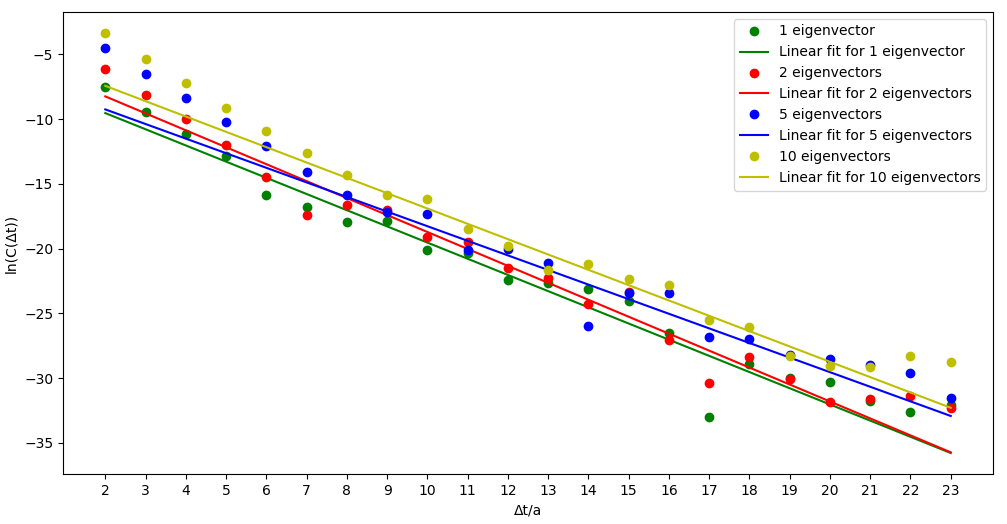
\includegraphics[width=1\textwidth]{images/1_2_5_10_evs_log.png}
        \caption{Combined results for 1, 2, 5 and 10 eigenvectors}
        \label{1_2_5_10_evs_log}
    \end{figure}
    
    \noindent
    In all computations the following creation operator was used:
    \begin{equation}
        \Operator(t) = \bar{\chi}^{(c)}(t)\gamma_5\chi^{(c)}(t)
    \end{equation}
    Therefore the resulting meson has quantum numbers $0(0^-)$ \cite{masses_of_D_mesons}. This was achieved by using for both propagators $(D^{-1(f)})$ the same flavor $f$. This approach reduced the amount of inversions that had to be calculated significantly. For the same reason a charmonium state was chosen in contrast to e.g. the calculation of a pion mass. Inversions for particles with higher masses converge significantly faster.
    
    To compute the mass of the charmonium state the mean value of all configurations for one value of $\Delta t$ were computed and a simple linear function was fitted to $ln(C(\Delta t))$. The results for 1, 2, 5 and 10 eigenvectors can be seen in figure \ref{1_2_5_10_evs_log}. One can see the similar shapes of all four results. Because the exponential nature of the correlation function only holds for $\Delta t \rightarrow \infty$ only a few points were chosen to be fitted. In figure \ref{1_2_5_10_evs_log_separate} one can see the four results side by side. The points which were used to fit the linear function are colored differently.
    
    The masses of these four simulations are shown in table \ref{meson_masses}, the errors were calculated using the \textit{Jackknife} \cite{jackknife} method.
    \begin{table}[h]
            \centering
            \begin{tabular}{|c|c|}
            \hline
            \multicolumn{1}{|c|}{Number of eigenvectors} & \multicolumn{1}{c|}{Mass (MeV)} \\ \hline
             1 & $3082 \pm 255$\\
             2 & $3227 \pm 215$\\
             5 & $2780 \pm 91$\\
             10& $2919 \pm 88$\\
              \hline
            \end{tabular}
            \caption{Calculated masses for the charmonium state}
            \label{meson_masses}
        \end{table}
    
    
    
    \begin{figure}[H]
        \centering
        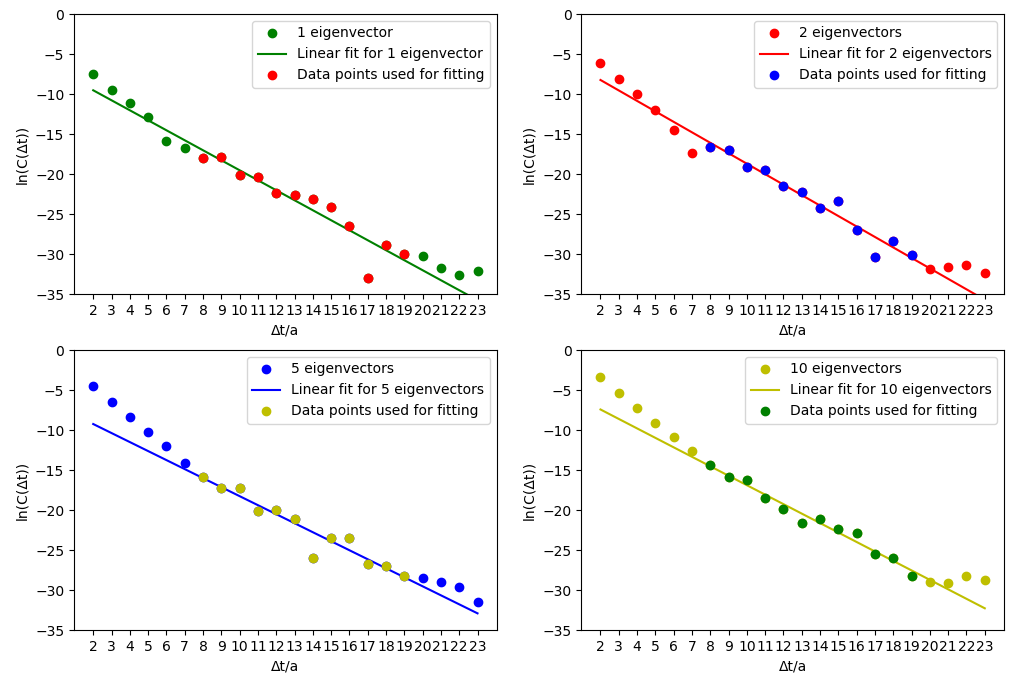
\includegraphics[width=1\textwidth]{images/1_2_5_10_evs_side.png}
        \caption{Logarithmic results for 1, 2, 5 and 10 eigenvectors. The data points used for fitting are colored differently.}
        \label{1_2_5_10_evs_log_separate}
    \end{figure}
	
	\section{Discussion}
	
	This work represents a first test of distillation by Marc Wagner's work group, therefore the number of eigenvectors and gauge configurations was kept small.\\
The results do show that calculating meson masses using distillation is feasable. Even using such a limited number of gauge configurations produced a value close to that in the literature. To improve accuracy a higher number of configuration should be used. Looking at the different number of eigenvectors a trend towards more precise calculations can be seen. While increasing the number of configurations increases simulation times linearly, a higher number of eigenvectors will increase times quadratically.\\
Testing the effect of a higher number of gauge configurations I could observe an improvement in accuracy when doubling the number of configurations similar to that of doubling the number of eigenvectors. In conclusion it seems advisable to increase the number of configurations at twice the "speed" (??) in regards to the number of eigenvectors.
	
	\newpage
	\bibliography{ref}
	

\end{document}